% test-cles-graph.tex -- test exhaustif des clés de tkz-graph (et tkz-berge)
% À compiler avec l'ancienne version (xkeyval) puis la nouvelle (pgfkeys) :
% les PDF doivent être identiques (vérifié le 2026/10/07, 4 pages).
% Les versions de développement sont trouvées par les liens de ~/Library/texmf.
\documentclass{article}
\usepackage[margin=1cm]{geometry}
\usepackage{tkz-graph}
\usepackage{tkz-berge}
\usetikzlibrary{shapes.geometric,positioning}
\pagestyle{empty}
\begin{document}
\section*{1. vstyle}
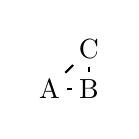
\begin{tikzpicture}[scale=.5]
  \GraphInit[vstyle=Empty]
  \Vertex{A}\EA(A){B}\NO(B){C}
  \Edges(A,B,C,A)
\end{tikzpicture}\quad
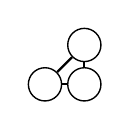
\begin{tikzpicture}[scale=.5]
  \GraphInit[vstyle=Hasse]
  \Vertex{A}\EA(A){B}\NO(B){C}
  \Edges(A,B,C,A)
\end{tikzpicture}\quad
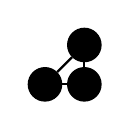
\begin{tikzpicture}[scale=.5]
  \GraphInit[vstyle=Simple]
  \Vertex{A}\EA(A){B}\NO(B){C}
  \Edges(A,B,C,A)
\end{tikzpicture}\quad
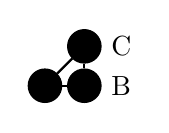
\begin{tikzpicture}[scale=.5]
  \GraphInit[vstyle=Classic]
  \Vertex{A}\EA(A){B}\NO(B){C}
  \Edges(A,B,C,A)
\end{tikzpicture}\quad
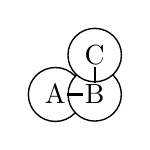
\begin{tikzpicture}[scale=.5]
  \GraphInit[vstyle=Normal]
  \Vertex{A}\EA(A){B}\NO(B){C}
  \Edges(A,B,C,A)
\end{tikzpicture}\quad
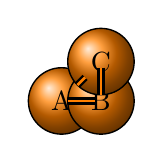
\begin{tikzpicture}[scale=.5]
  \GraphInit[vstyle=Shade]
  \Vertex{A}\EA(A){B}\NO(B){C}
  \Edges(A,B,C,A)
\end{tikzpicture}\quad
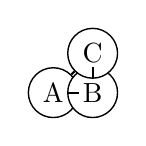
\begin{tikzpicture}[scale=.5]
  \GraphInit[vstyle=Dijkstra]
  \Vertex{A}\EA(A){B}\NO(B){C}
  \Edges(A,B,C,A)
\end{tikzpicture}\quad
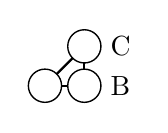
\begin{tikzpicture}[scale=.5]
  \GraphInit[vstyle=Welsh]
  \Vertex{A}\EA(A){B}\NO(B){C}
  \Edges(A,B,C,A)
\end{tikzpicture}\quad
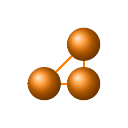
\begin{tikzpicture}[scale=.5]
  \GraphInit[vstyle=Art]
  \Vertex{A}\EA(A){B}\NO(B){C}
  \Edges(A,B,C,A)
\end{tikzpicture}\quad
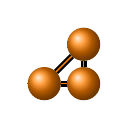
\begin{tikzpicture}[scale=.5]
  \GraphInit[vstyle=Shade Art]
  \Vertex{A}\EA(A){B}\NO(B){C}
  \Edges(A,B,C,A)
\end{tikzpicture}\quad


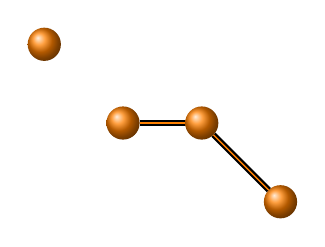
\begin{tikzpicture}[scale=.5]
  \GraphInit[vstyle=shade art,unit=2]   % casse indifférente, unit
  \Vertex{A}\EA(A){B}\SOEA(B){C}\NOWE(A){D}
  \Edges(A,B,C)
\end{tikzpicture}
% (deux \GraphInit dans le même groupe : voir test-graphinit.tex)

\section*{2. SetVertexSimple, Shade, Art, Normal}
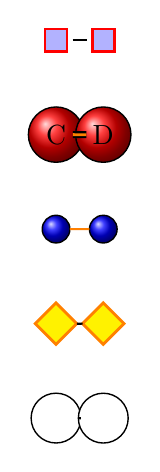
\begin{tikzpicture}[scale=.6]
  \SetVertexSimple[Shape=rectangle,MinSize=8pt,LineWidth=1pt,LineColor=red,
                   FillColor=blue!30,InnerSep=1pt,OuterSep=2pt]
  \Vertex{A}\EA(A){B}\Edge(A)(B)
  \SetVertexShade[Shape=circle,MinSize=20pt,LineWidth=.2pt,LineColor=green,
                  BallColor=red,InnerSep=3pt,OuterSep=1pt]
  \Vertex[x=0,y=-2]{C}\EA(C){D}\Edge(C)(D)
  \SetVertexArt[MinSize=10pt,BallColor=blue]
  \Vertex[x=0,y=-4]{E}\EA(E){F}\Edge(E)(F)
  \SetVertexNormal[Shape=diamond,MinSize=15pt,LineWidth=1pt,LineColor=orange,
                   FillColor=yellow,TextColor=red,InnerSep=2pt,OuterSep=0pt]
  \Vertex[x=0,y=-6]{G}\EA(G){H}\Edge(G)(H)
  \SetVertexNormal
  \Vertex[x=0,y=-8]{I}\EA(I){J}\Edge(I)(J)
\end{tikzpicture}

\section*{3. Vertex}
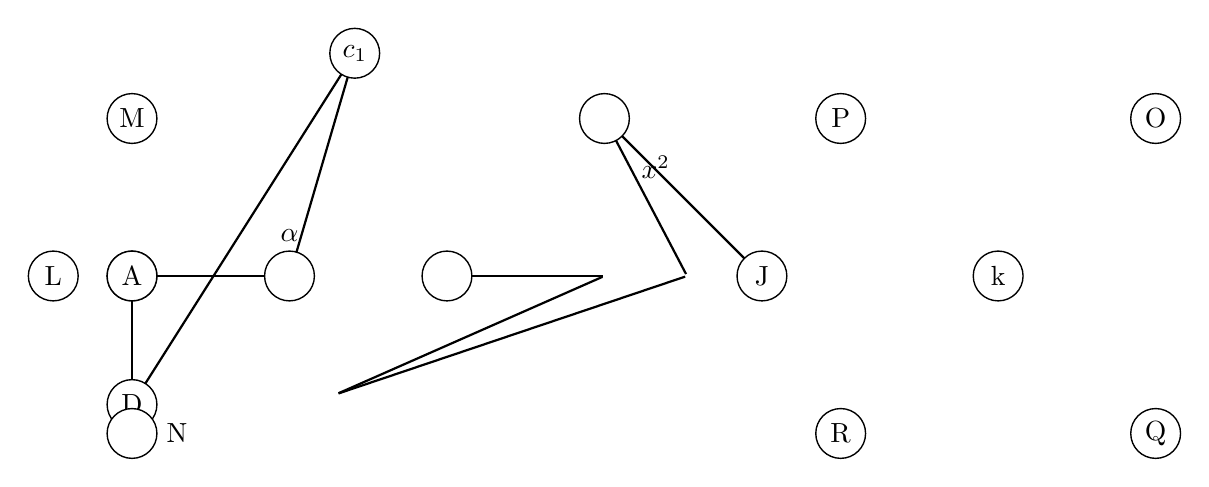
\begin{tikzpicture}
  \SetGraphUnit{2}
  \Vertex{A}
  \Vertex[x=2,y=0,L=$\alpha$,Lpos=90,LabelOut]{B}
  \Vertex[a=45,d=4,Math]{c_1}
  \Vertex[position={below=of A},style={fill=red!20}]{D}
  \Vertex[x=4,y=0,NoLabel]{E}
  \Vertex[x=6,y=0,empty]{F}
  \Vertex[a=-30,d=3,empty]{G}
  \Vertex[position={right=1cm of F},empty]{H}
  \Vertex[x=6,y=2,LabelOut,Lpos=-45,Ldist=5pt,Math,L=x^2]{I}
  \Vertex[x=8,y=0,LabelOut=false,NoLabel=false]{J}
  \Edges(A,B,c_1,D,A)\Edges(E,F,G,H,I,J)
  \Vertex[Node]{A}
  \EA[unit=3,L=k](J){K}\WE[unit=1](A){L}\NO(A){M}\SO[Lpos=0,LabelOut](A){N}
  \NOEA(K){O}\NOWE(K){P}\SOEA(K){Q}\SOWE(K){R}
\end{tikzpicture}

\section*{4. SetUpVertex et présélections}
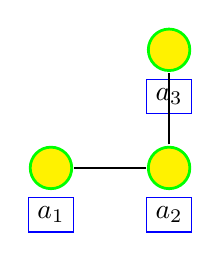
\begin{tikzpicture}
  \SetUpVertex[Lpos=-90,Ldist=2pt,Style={draw=blue},MinSize=15pt,LineWidth=1pt,
     TextColor=red,LineColor=green,FillColor=yellow,InnerSep=1pt,OuterSep=1pt,
     Unit=1.5,LabelOut,Math]
  \Vertex{a_1}\EA(a_1){a_2}\NO(a_2){a_3}
  \Edges(a_1,a_2,a_3)
\end{tikzpicture}
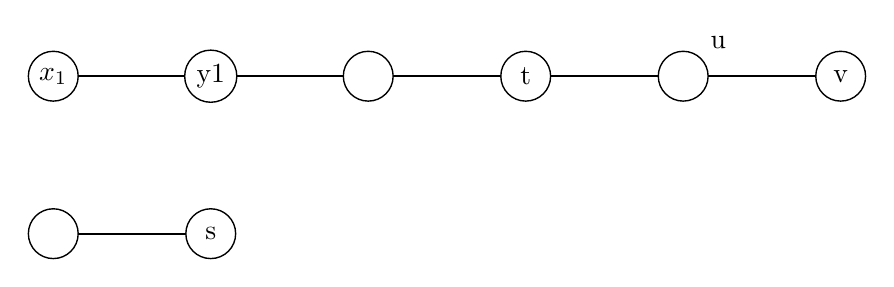
\begin{tikzpicture}
  \SetVertexMath\Vertex{x_1}\SetVertexNoMath\Vertex[x=2,y=0]{y1}
  \SetVertexNoLabel\Vertex[x=4,y=0]{z}\SetVertexLabel\Vertex[x=6,y=0]{t}
  \SetVertexLabelOut\Vertex[x=8,y=0,Lpos=45]{u}\SetVertexLabelIn\Vertex[x=10,y=0]{v}
  \begingroup\SetVertexNoLabel\Vertex[x=0,y=-2]{w}\endgroup
  \Vertex[x=2,y=-2]{s}  % le groupe limite la présélection
  \Edges(x_1,y1,z,t,u,v)\Edge(w)(s)
\end{tikzpicture}

\section*{5. Vertices}
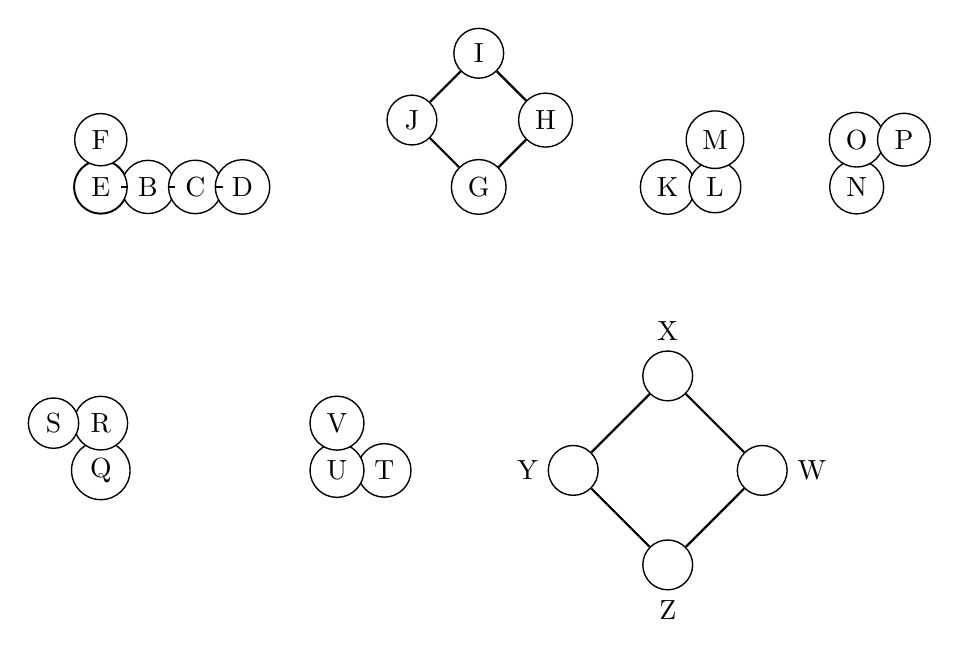
\begin{tikzpicture}[scale=.6]
  \GraphInit[vstyle=Normal]
  \Vertices{line}{A,B,C,D}
  \Vertices[y=-2,dir=\NO]{line}{E,F}
  \begin{scope}[xshift=8cm]\Vertices[unit=2]{square}{G,H,I,J}\end{scope}
  \begin{scope}[xshift=12cm]\Vertices{tr1}{K,L,M}\end{scope}
  \begin{scope}[xshift=16cm]\Vertices{tr2}{N,O,P}\end{scope}
  \begin{scope}[yshift=-6cm]\Vertices{tr3}{Q,R,S}\end{scope}
  \begin{scope}[yshift=-6cm,xshift=6cm]\Vertices{tr4}{T,U,V}\end{scope}
  \begin{scope}[yshift=-6cm,xshift=12cm]
     \Vertices[unit=2,LabelOut,Lpos=0]{circle}{W,X,Y,Z}\end{scope}
  \Edges(A,B,C,D)\Edges(G,H,I,J,G)\Edges(W,X,Y,Z,W)
\end{tikzpicture}

\section*{6. Edge, Edges, SetUpEdge}
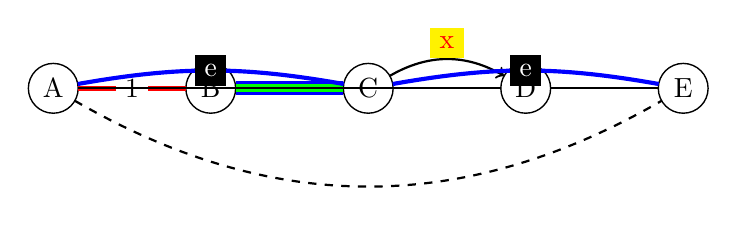
\begin{tikzpicture}
  \SetGraphUnit{2}
  \Vertex{A}\EA(A){B}\EA(B){C}\EA(C){D}\EA(D){E}
  \Edge[color=red,lw=2pt,label=$1$](A)(B)
  \Edge[double=blue,incolor=yellow,dd=1pt,lw=3pt,color=green](B)(C)
  \Edge[style={bend left,->},label=x,labeltext=red,labelcolor=yellow,
        labelstyle={above}](C)(D)
  \tikzset{EdgeStyle/.style={dashed}}
  \Edge[local](D)(E)
  \Edge[style={bend right}](A)(E)
  \tikzset{EdgeStyle/.style={}}
  \SetUpEdge[color=blue,lw=1.5pt,label=e,labeltext=white,labelcolor=black,
             labelstyle={sloped},style={bend left=10}]
  \Edges(A,C,E)
  \SetUpEdge
  \Edges[color=orange](B,D)
  \DisableEdgeStyle
  \Edge(A)(D)
\end{tikzpicture}

\section*{7. Loop}
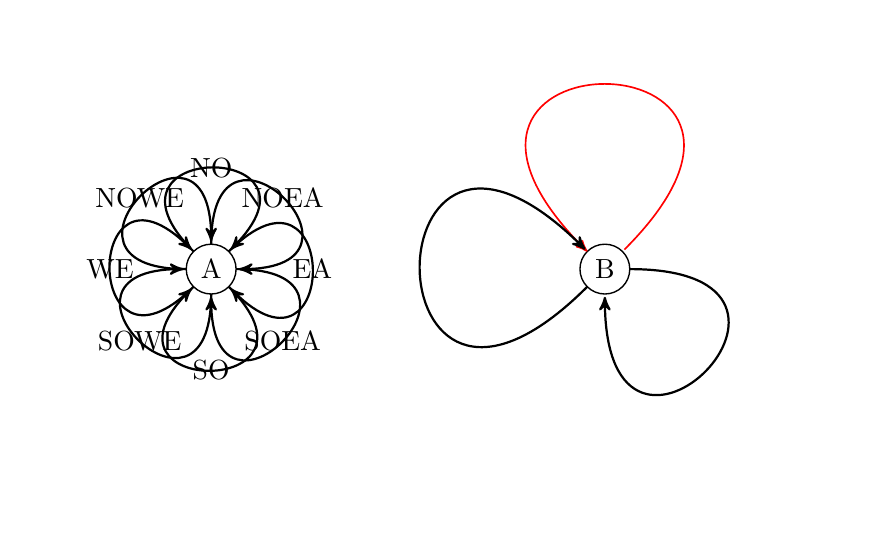
\begin{tikzpicture}
  \Vertex{A}
  \Loop[dir=WE,dist=2cm,label=WE](A)
  \Loop[dir=EA,dist=2cm,label=EA](A)
  \Loop[dir=NO,dist=2cm,label=NO](A)
  \Loop[dir=SO,dist=2cm,label=SO](A)
  \Loop[dir=NOWE,dist=2cm,label=NOWE](A)
  \Loop[dir=NOEA,dist=2cm,label=NOEA](A)
  \Loop[dir=SOWE,dist=2cm,label=SOWE](A)
  \Loop[dir=SOEA,dist=2cm,label=SOEA](A)
  \Vertex[x=5,y=0]{B}
  \Loop[dir=no,color=red,style={post},labelstyle={above}](B)
  \Loop[dir=soEA,dist=3cm](B)
  \Loop(B)
\end{tikzpicture}
\begin{tikzpicture}
  \Vertex{A}\grLoop[dir=EA,label=$1/2$,labelstyle={right}](A)
\end{tikzpicture}

\section*{8. Graphes probabilistes}
\begin{tikzpicture}
  \grProb{A}{B}{0,3}{0,4}{0,7}{0,6}
\end{tikzpicture}
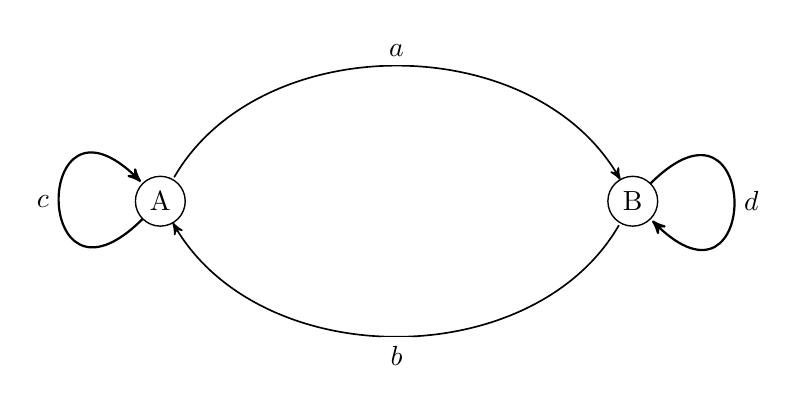
\begin{tikzpicture}
  \grProb[unit=6,LposA=90,LposB=-90,Ldist=3pt,LoopDist=2cm]{A}{B}{a}{b}{c}{d}
\end{tikzpicture}

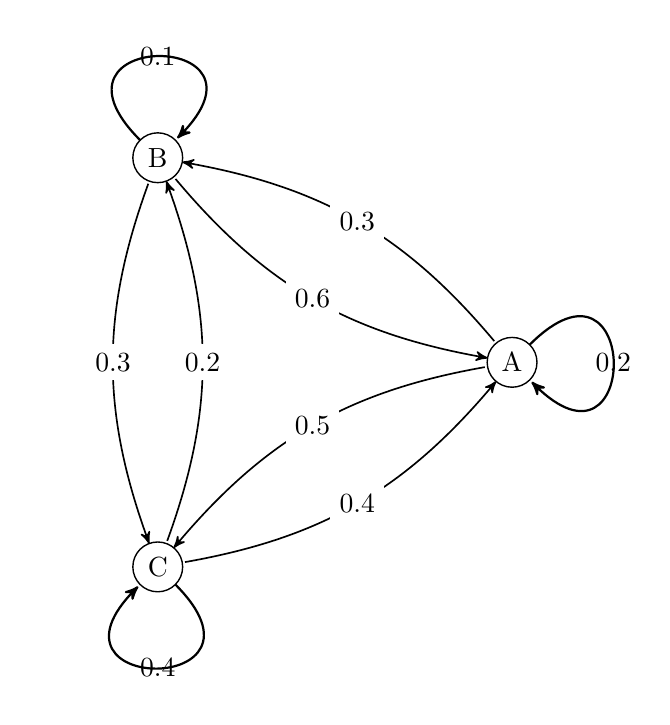
\begin{tikzpicture}
  \grProbThree[unit=3,LoopDist=2cm]{A}{B}{C}{0.2/0.3/0.5}{0.1/0.6/0.3}{0.4/0.4/0.2}
\end{tikzpicture}

\section*{9. Couleurs et styles prédéfinis}
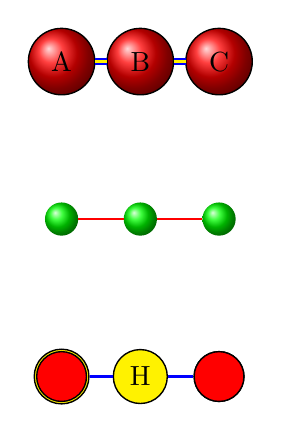
\begin{tikzpicture}
  \begin{scope}\GraphInit[vstyle=Shade]\SetGraphShadeColor{red}{blue}{yellow}
  \Vertices{line}{A,B,C}\Edges(A,B,C)\end{scope}
  \begin{scope}[yshift=-2cm]\GraphInit[vstyle=Art]\SetGraphArtColor{green}{red}
  \Vertices{line}{D,E,F}\Edges(D,E,F)\end{scope}
  \begin{scope}[yshift=-4cm]\GraphInit[vstyle=Normal]\SetGraphColor{yellow}{blue}
  \Vertices{line}{G,H,I}\Edges(G,H,I)
  \AddVertexColor{red}{G,I}\end{scope}
\end{tikzpicture}
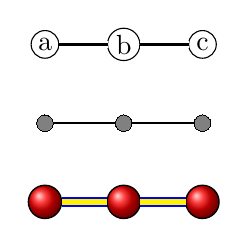
\begin{tikzpicture}
  \begin{scope}\SetVertexLabeledSmall\Vertices{line}{a,b,c}\Edges(a,b,c)\end{scope}
  \begin{scope}[yshift=-1cm]\SetVertexNotLabeledSmall\Vertices{line}{d,e,f}\Edges(d,e,f)\end{scope}
  \begin{scope}[yshift=-2cm]\SetVertexForPresentation{red}{blue}{yellow}\Vertices{line}{g,h,i}\Edges(g,h,i)\end{scope}
\end{tikzpicture}
\tkzSetUpColors[background=white,text=black]

\section*{10. tkz-berge}
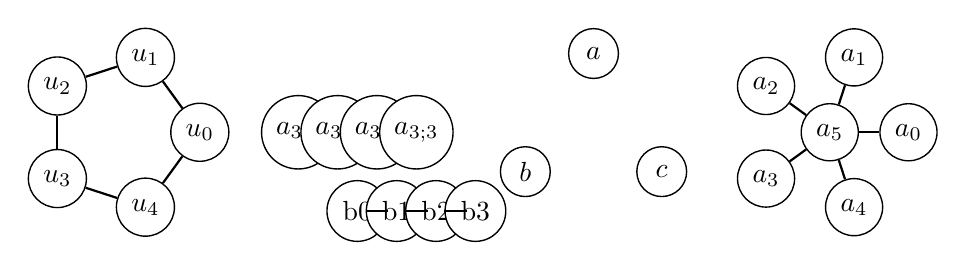
\begin{tikzpicture}[scale=.5]
  \GraphInit[vstyle=Normal]
  \grEmptyCycle[RA=2,prefix=u,Math]{5}
  \EdgeInGraphLoop[color=red]{u}{5}
  \begin{scope}[xshift=6cm]
    \grEmptyPath[form=2,RA=1,Math,num=3]{4}
    \grEmptyPath[form=1,RA=1,y=-2,prefix=b]{4}
    \EdgeInGraphSeq[lw=2pt]{b}{0}{2}
  \end{scope}
  \begin{scope}[xshift=12cm]
    \grEmptyCycle*[RA=2,rotation=90,Math]{a,b,c}
  \end{scope}
  \begin{scope}[xshift=18cm]
    \grEmptyStar[RA=2,Math]{6}\EdgeFromOneToAll{a}{a}{5}{5}
  \end{scope}
\end{tikzpicture}

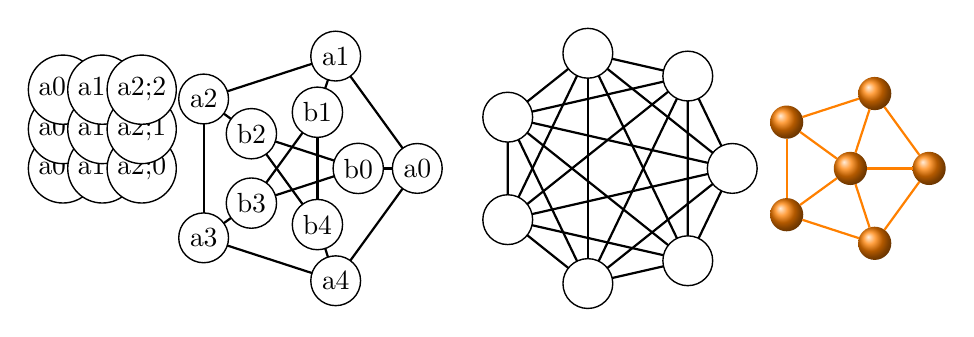
\begin{tikzpicture}[scale=.5]
  \grEmptyGrid[RA=1,RB=1]{3}{3}
  \begin{scope}[xshift=6cm]\grPetersen[RA=3,RB=1.5]\end{scope}
  \begin{scope}[xshift=14cm]
    \SetVertexNoLabel\grComplete[RA=3,x=0,y=0]{7}\end{scope}
  \begin{scope}[xshift=20cm]
    \GraphInit[vstyle=Art]\grWheel[RA=2,prefix=x,prefixx=y]{6}\end{scope}
\end{tikzpicture}

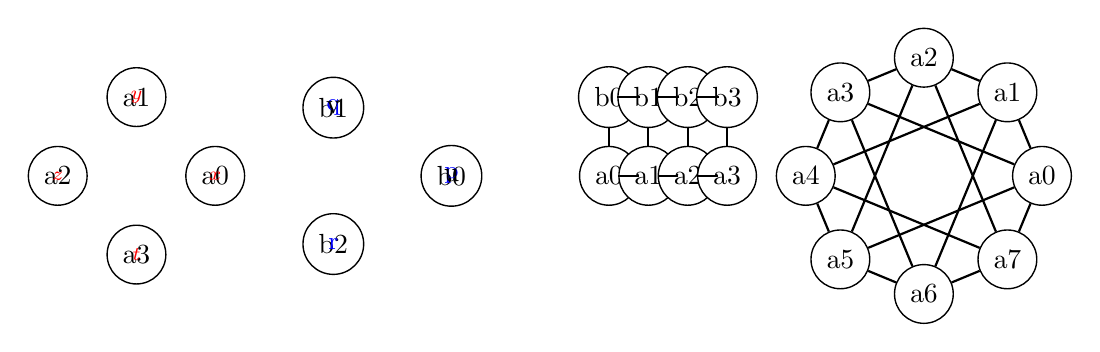
\begin{tikzpicture}[scale=.5]
  \GraphInit[vstyle=Normal]\SetVertexLabel
  \grEmptyCycle[RA=2]{4}
  \AssignVertexLabel[color=red,Math,mathsize=\scriptstyle]{a}{x,y,z,t}
  \begin{scope}[xshift=6cm]
    \grEmptyCycle[RA=2,prefix=b]{3}
    \AssignVertexLabel[size=\small,color=blue]{b}{p,q,r}
    \grWriteExplicitLabels[color=red]{u/b0,v/b1}
  \end{scope}
  \begin{scope}[xshift=12cm]
    \grLadder[RA=1,RS=2]{4}
  \end{scope}
  \begin{scope}[xshift=20cm]
    \grCirculant[RA=3]{8}{1,3}
  \end{scope}
\end{tikzpicture}
\end{document}
